% !TeX encoding = UTF-8
\documentclass[aspectratio=169]{beamer}
\useoutertheme[progressbar=frametitle]{metropolis}
\useinnertheme{metropolis}
\definecolor{nabgray}{rgb}{0.6,0.59,0.61}
\usecolortheme[named=nabgray]{structure}

\usepackage{tikz}
\usepackage[utf8]{inputenc}
\usepackage[spanish]{babel}

\usepackage{smartdiagram}
\usepackage{qtree}
\usepackage{verbatim}
\usepackage{svg}
\usepackage{graphicx}
\usepackage{color}


\definecolor{lightgray}{rgb}{0.95, 0.95, 0.95}
\definecolor{darkgray}{rgb}{0.4, 0.4, 0.4}
%\definecolor{purple}{rgb}{0.65, 0.12, 0.82}
\definecolor{editorGray}{rgb}{0.95, 0.95, 0.95}
\definecolor{editorOcher}{rgb}{1, 0.5, 0} % #FF7F00 -> rgb(239, 169, 0)
\definecolor{editorGreen}{rgb}{0, 0.5, 0} % #007C00 -> rgb(0, 124, 0)
\definecolor{orange}{rgb}{1,0.45,0.13}
\definecolor{olive}{rgb}{0.17,0.59,0.20}
\definecolor{brown}{rgb}{0.69,0.31,0.31}
\definecolor{purple}{rgb}{0.38,0.18,0.81}
\definecolor{lightblue}{rgb}{0.1,0.57,0.7}
\definecolor{lightred}{rgb}{1,0.4,0.5}
\definecolor{ocherCode}{rgb}{1, 0.5, 0} % #FF7F00 -> rgb(239, 169, 0)
\definecolor{blueCode}{rgb}{0, 0, 0.93} % #0000EE -> rgb(0, 0, 238)
\definecolor{greenCode}{rgb}{0, 0.6, 0} % #009900 -> rgb(0, 153, 0)


\usepackage{upquote}
\usepackage{listings}
\lstdefinelanguage{JavaScript}{
    morekeywords=[1]{break, continue, delete, else, for, function, if, in,
        new, return, this, typeof, var, void, while, with},
    % Literals, primitive types, and reference types.
    morekeywords=[2]{false, null, true, boolean, number, undefined,
        Array, Boolean, Date, Math, Number, String, Object},
    % Built-ins.
    morekeywords=[3]{eval, parseInt, parseFloat, escape, unescape},
    % Basic design
    backgroundcolor=\color{lightgray},
    basicstyle={\small\ttfamily},
    frame=l,
    keywordstyle=\footnotesize\color{blue},
    escapeinside={<@}{@>},
    breaklines=true,
    % Line numbers
    xleftmargin={0.75cm},
    numbers=left,
    stepnumber=1,
    firstnumber=1,
    numberfirstline=true
    % Code design
    identifierstyle=\color{black},
    keywordstyle=\color{ocherCode}\bfseries,
    ndkeywordstyle=\color{greenCode}\bfseries,
    stringstyle=\color{ocherCode}\ttfamily,
    commentstyle=\color{darkgray}\ttfamily,
    tabsize=2,
    showtabs=true,
    showspaces=false,
    showstringspaces=false,
    extendedchars=true,
    breaklines=true
}[keywords, comments, strings]

\colorlet{punct}{red!60!black}
\definecolor{background}{HTML}{EEEEEE}
\definecolor{delim}{RGB}{20,105,176}
\colorlet{numb}{magenta!60!black}

\lstdefinelanguage{json}{
    basicstyle=\normalfont\ttfamily,
    numbers=left,
    numberstyle=\scriptsize,
    stepnumber=1,
    numbersep=8pt,
    showstringspaces=false,
    breaklines=true,
    frame=lines,
    literate=
    *{0}{{{\color{numb}0}}}{1}
    {1}{{{\color{numb}1}}}{1}
    {2}{{{\color{numb}2}}}{1}
    {3}{{{\color{numb}3}}}{1}
    {4}{{{\color{numb}4}}}{1}
    {5}{{{\color{numb}5}}}{1}
    {6}{{{\color{numb}6}}}{1}
    {7}{{{\color{numb}7}}}{1}
    {8}{{{\color{numb}8}}}{1}
    {9}{{{\color{numb}9}}}{1}
    {:}{{{\color{punct}{:}}}}{1}
    {,}{{{\color{punct}{,}}}}{1}
    {\{}{{{\color{delim}{\{}}}}{1}
    {\}}{{{\color{delim}{\}}}}}{1}
    {[}{{{\color{delim}{[}}}}{1}
    {]}{{{\color{delim}{]}}}}{1},
}
\lstset{language=java,
    basicstyle=\footnotesize\ttfamily,
    keywordstyle=\footnotesize\color{blue}\ttfamily,
}


\usebackgroundtemplate%
{%
    
\includegraphics[width=\paperwidth]{Images/Contenido}%
}


\title{Gestión de proyectos con Maven}
\author{Víctor Orozco - @tuxtor}
\institute{Academik}
\date{\today}

\begin{document}

{
    \usebackgroundtemplate{
\includegraphics[width=\paperwidth]{Images/portada}}
    \setbeamercolor{frametitle}{fg=red}
    \usebeamercolor[fg]{normal text}
    \frame{\titlepage}
}



\begin{frame}{¿Como programar en Java?}
\begin{enumerate}
	\item Crear un proyecto (Objetivo, framework y SCM)
	\item Programar el proyecto
	\item Ejecutar el proyecto*
\end{enumerate}
\end{frame}

\begin{frame}{¿Como programar en Java?}
\begin{enumerate}
	\item \textbf{Crear un proyecto (Objetivo, framework y SCM)}
	\item Programar el proyecto
	\item Ejecutar el proyecto*
\end{enumerate}
\end{frame}

{
    \usebackgroundtemplate{
\includegraphics[width=\paperwidth]{Images/separador}}
    \setbeamercolor{normal text}{fg=white}
    \setbeamercolor{frametitle}{fg=red}
    \usebeamercolor[fg]{normal text}
    \section{Proyectos en Maven}
}



\begin{frame}{Compilador}
\begin{figure}
	\centering
	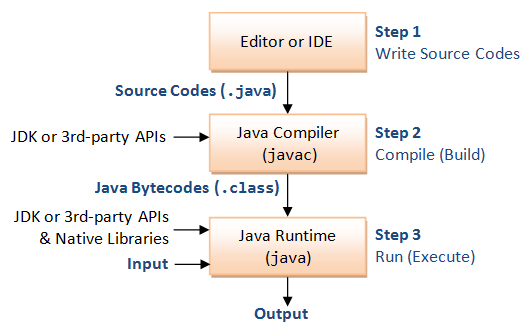
\includegraphics[width=0.8\linewidth]{Images/javac2}
\end{figure}
\end{frame}


\begin{frame}{Compilador}
\begin{figure}
	\centering
	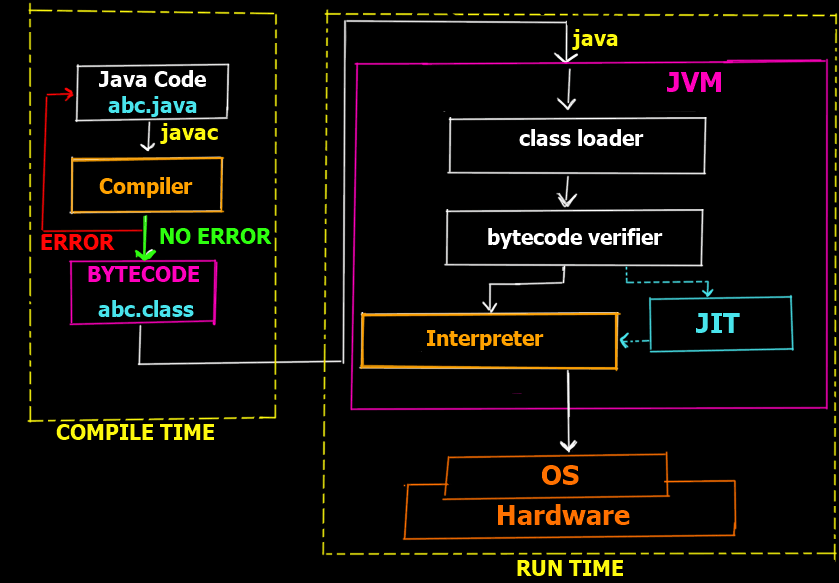
\includegraphics[width=0.7\linewidth]{Images/javac1}
\end{figure}
\end{frame}


\begin{frame}{Compilador}
\begin{itemize}
	\item ¿Dependencias?
	\item ¿Proceso de ensamblaje?
	\item ¿Proyecto final? ¿.jar, .war, .ear
\end{itemize}
\pause
Task runner + Gestor de dependencias
\end{frame}

\begin{frame}{Maven}
\begin{itemize}
	\item Project Object Model (Declarativo)
	\item Construcción, reportes, documentación
	\item Build tool
	\item Arquetipos
	\item Ensamblado manual
	\item Bill of materials (BOM)
	\item Starter
	\item .jar, .war, .ear
\end{itemize}
\end{frame}


\begin{frame}{Maven - Arquetipo}
\begin{itemize}
	\item groupId: Identifica y da pertenencia al paquete/biblioteca/proyecto hacia una empresa/organización
	\item artifactId: Identificador primario del artefacto
	\item version: Versión del paquete
\end{itemize}
\end{frame}

\begin{frame}[fragile]{Maven - Arquetipo}
\begin{lstlisting}[language=bash]
mvn archetype:generate
    -DgroupId=com.nabenik -DartifactId=demo1
\end{lstlisting}
\end{frame}

\begin{frame}{Maven - Arquetipo}
\begin{figure}
	\centering
	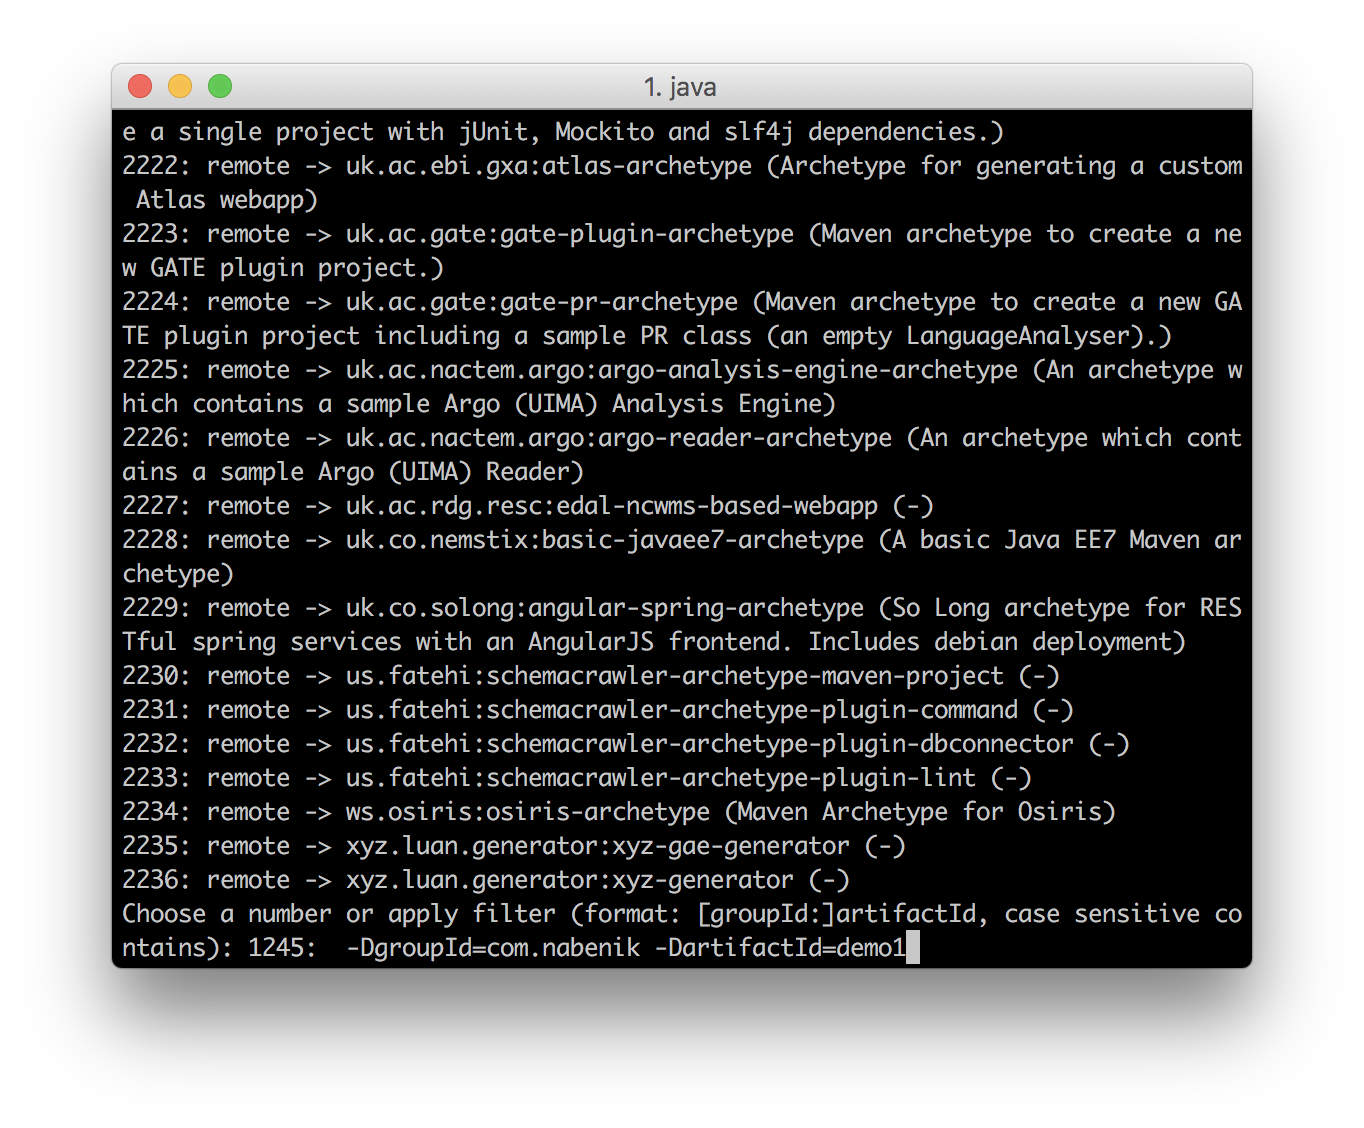
\includegraphics[width=\linewidth]{Images/mvn}
\end{figure}
\end{frame}

\begin{frame}[fragile]{Maven - Arquetipo}
\begin{lstlisting}[language=bash]
mvn archetype:generate -DgroupId=com.nabenik
    -DarchetypeArtifactId=maven-archetype-quickstart
    -DartifactId=demo1
\end{lstlisting}
\end{frame}

\begin{frame}{Maven - Arquetipo}
\begin{figure}
	\centering
	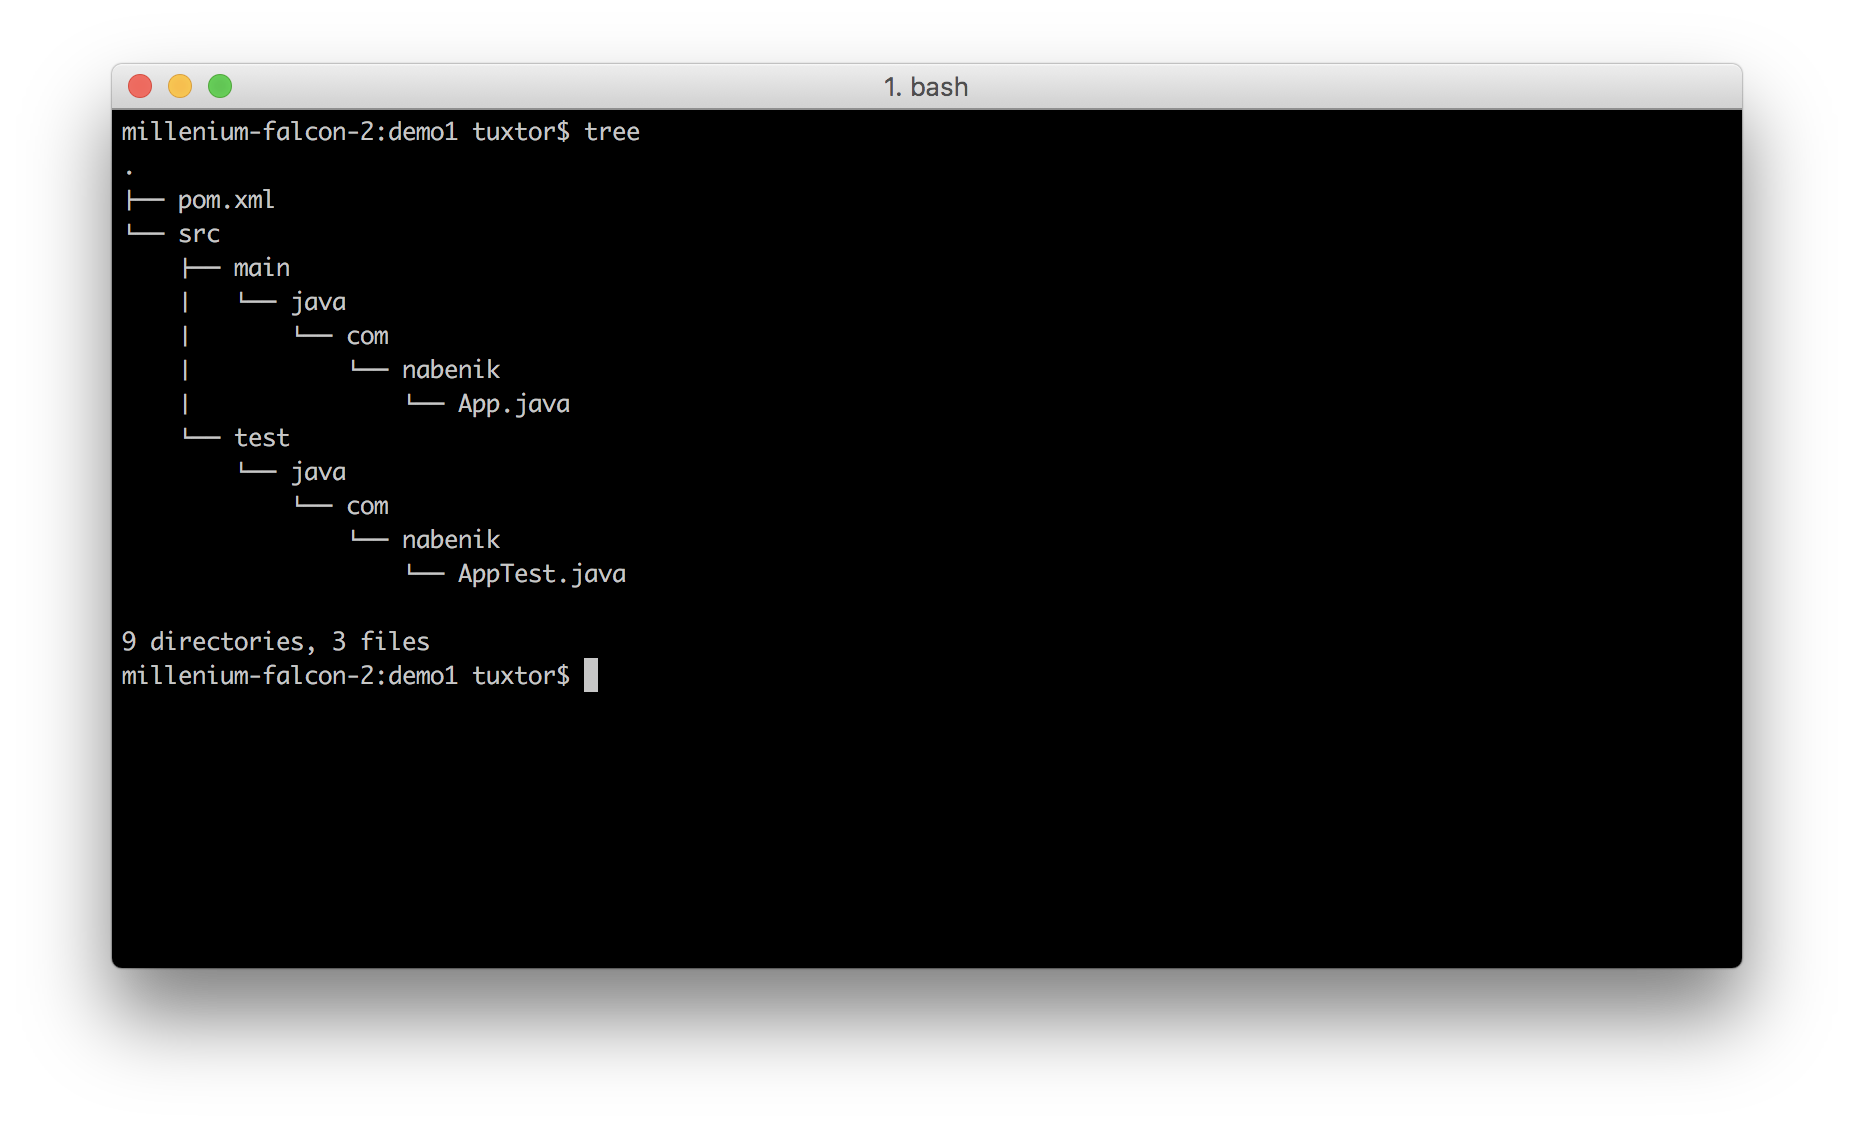
\includegraphics[width=\linewidth]{Images/mvn2}
\end{figure}
\end{frame}

\begin{frame}{Maven - Arquetipo}
Estructura de carpetas
\begin{itemize}
	\item src/main/java - Código fuente
	\item src/main/resources - Recursos del proyecto (se copian de forma integra)
	\item src/main/webapp - Recursos web y/o basados en Servlet
    \item src/test/* - Entorno de pruebas
    \item target - Archivos generados por Maven
\end{itemize}
\end{frame}

\begin{frame}{}
\begin{figure}
	\centering
	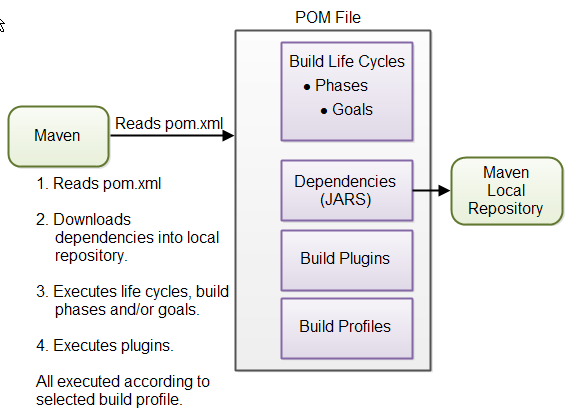
\includegraphics[width=0.8\linewidth]{Images/maven0}
\end{figure}
\end{frame}


\begin{frame}{}
\begin{figure}
	\centering
	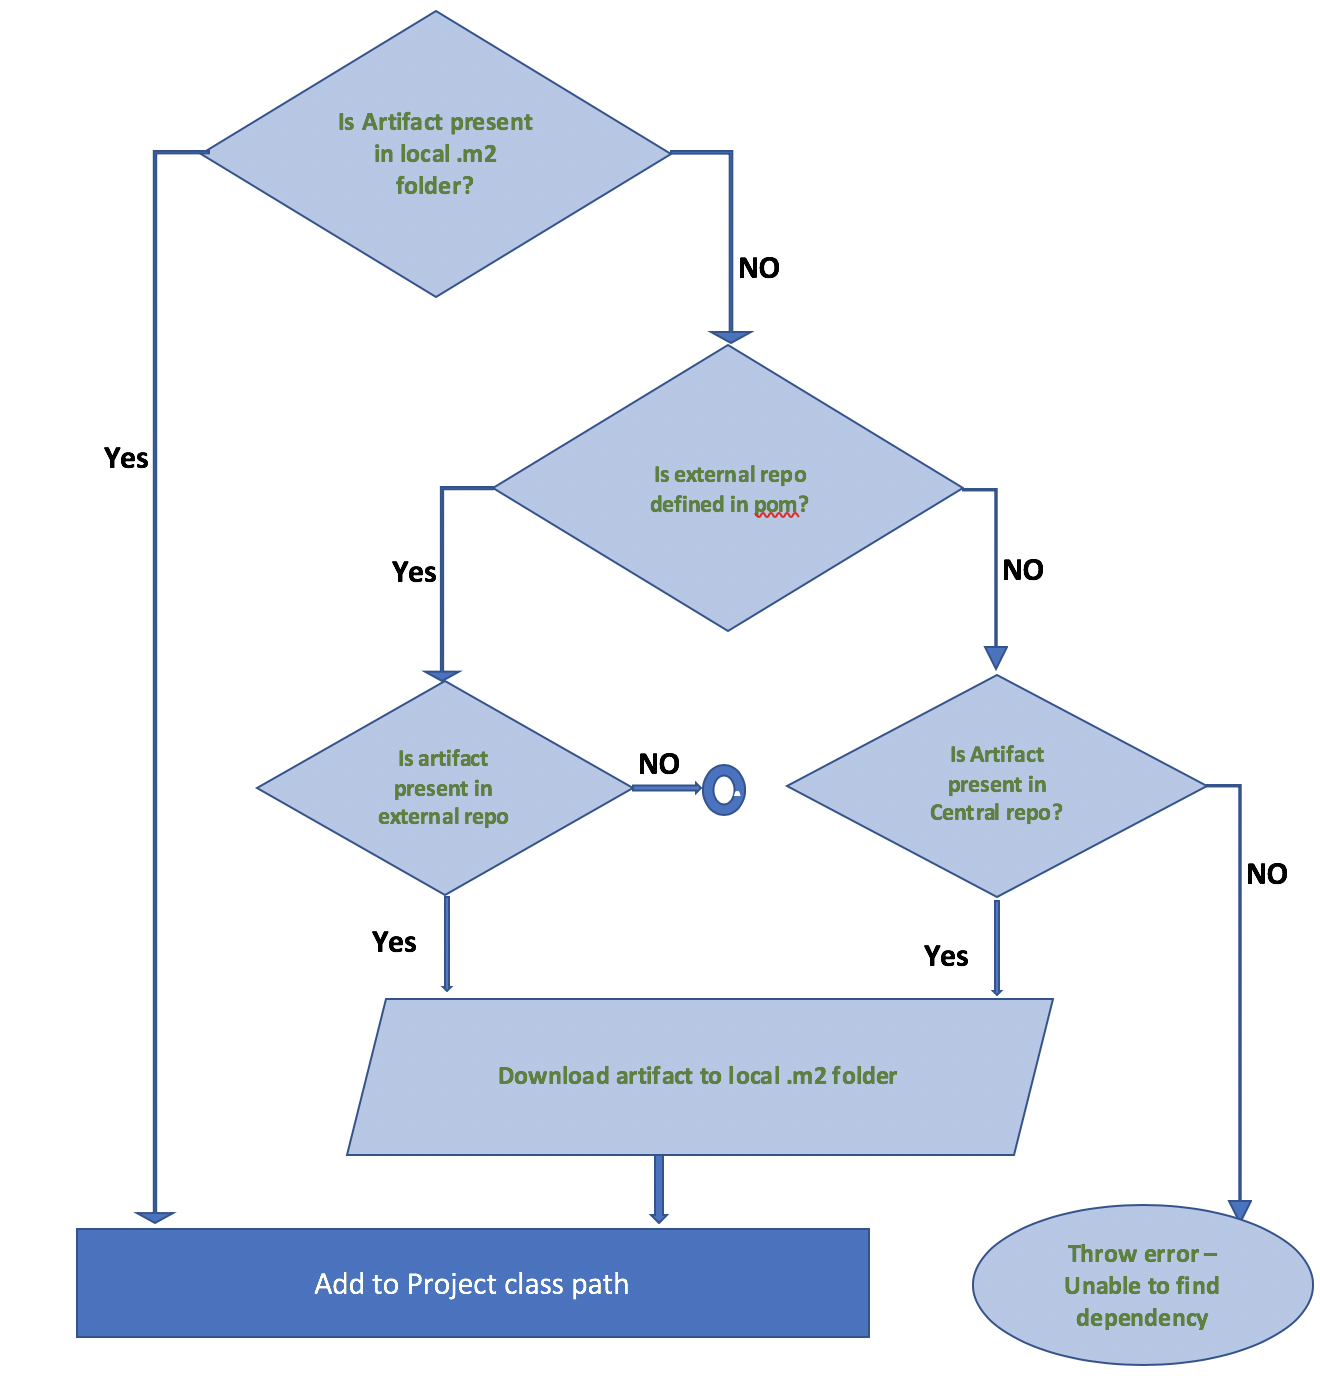
\includegraphics[width=0.6\linewidth]{Images/repomaven}
\end{figure}
\end{frame}

\begin{frame}{Maven}
\begin{figure}
	\centering
	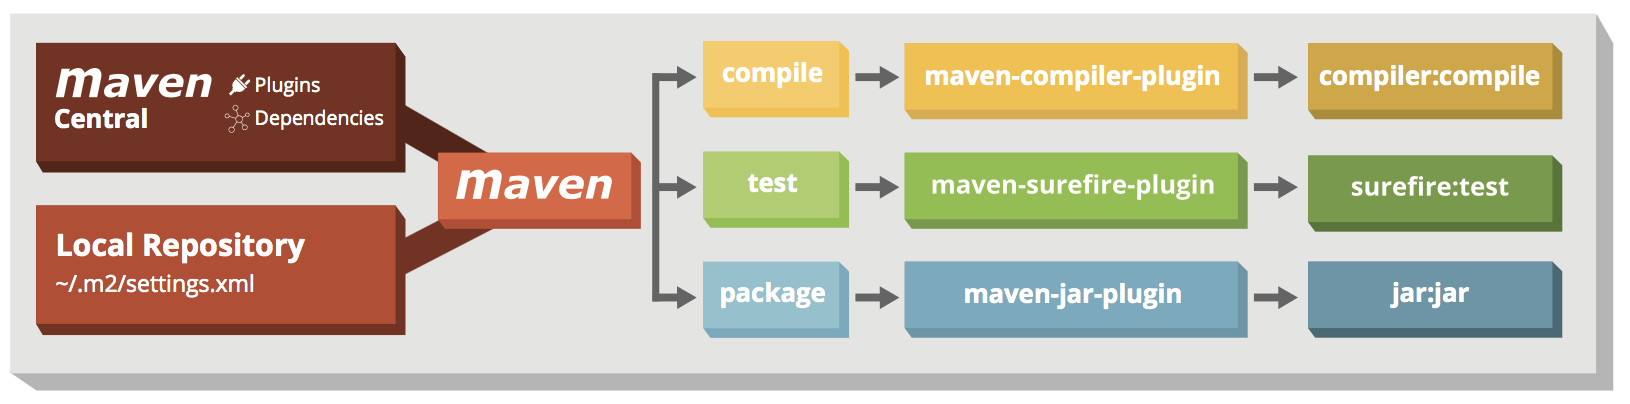
\includegraphics[width=0.9\linewidth]{Images/maven}
\end{figure}
\end{frame}

\begin{frame}{Maven - Fases}
\begin{itemize}
	\item \texttt{clean} - Elimina el directorio \texttt{target}
	\item \texttt{validate} - Valida si el proyecto es correcto
	\item \texttt{compile} - Compila los archivos fuente y almacena el resutado en \texttt{target/classes}
	\item  \texttt{test} - Ejecuta tests
	\item \texttt{package} - Toma los objetos compilados y los empaca en formatos distribuibles e.g. JAR, WAR
	\item \texttt{verify} - Ejecuta tests adicionales sobre el paquete para control de calidad
	\item \texttt{install} - Instala el paquete en el repositorio local
	\item \texttt{deploy} - Despliega el paquete en un repositorio remoto
\end{itemize}
\end{frame}


\begin{frame}{Maven - Ejercicio 1}

Mediante Maven ejecute la creación de un proyecto denominado demo2 y en el mismo implemente un programa que permita la fabricación de objetos automóvil de acuerdo al siguiente diagrama de clases:

\begin{figure}
	\centering
	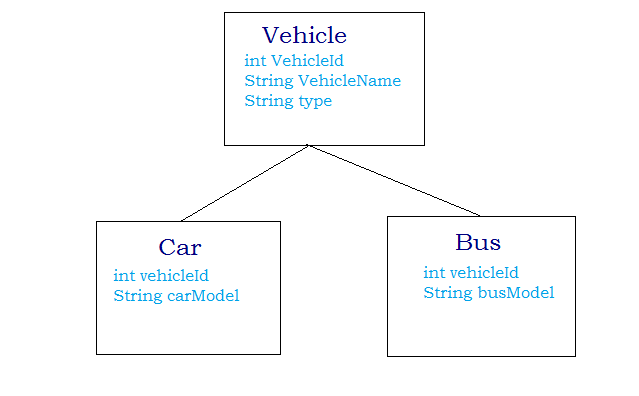
\includegraphics[width=0.7\linewidth]{Images/carro}
\end{figure}

\end{frame}


\begin{frame}[fragile]{Maven - Fases y plugins}
\begin{itemize}
	\item Fases - Ejecutadas por plugins intercambiables
	\item Goal - Un paso dentro de un plugin que se ejecuta dentro de una fase
	\item Los Goals ejecutan el trabajo dentro de las fases
\end{itemize}

\begin{lstlisting}[language=xml]
<build>
    <plugins>
    . . .
    </plugins>
</build>
\end{lstlisting}

\end{frame}

\begin{frame}[fragile]{Maven Plugins - Dependency}

\begin{lstlisting}[language=bash]
mvn dependency:analyze
\end{lstlisting}

\begin{lstlisting}[language=bash]
mvn dependency:tree
\end{lstlisting}
\end{frame}

\begin{frame}[fragile]{Maven Plugins - Compiler}

\begin{lstlisting}[language=xml]
<plugin>
    <groupId>org.apache.maven.plugins</groupId>
    <artifactId>maven-compiler-plugin</artifactId>
    <version>3.6.1</version>
    <configuration>
        <source>1.8</source>
        <target>1.8</target>
    </configuration>
</plugin>
\end{lstlisting}
\end{frame}

\begin{frame}[fragile]{Maven Plugins - Jar}

{\tiny
\begin{lstlisting}[language=xml]
<plugin>
    <groupId>org.apache.maven.plugins</groupId>
    <artifactId>maven-jar-plugin</artifactId>
    <version>3.1.0</version>
    ...
    <configuration>
        <archive>
            <manifest>
                <addClasspath>true</addClasspath>
                <mainClass>fully.qualified.MainClass</mainClass>
            </manifest>
        </archive>
    </configuration>
    ...
</plugin>
\end{lstlisting}
}
\end{frame}

\begin{frame}{Maven - Ejemplo 2}

Compile y empaque el proyecto, posteriormente ejecute la clase \texttt{App.java} contenida en el arquetipo de java

\end{frame}

\begin{frame}{Maven - Ejemplo 3}

Ejecute los ejercicios 1 y 2 en su IDE de preferencia

\end{frame}


\begin{frame}{Maven - Ejemplo 4}

Utilice el starter de Helidon para generar una API web con MicroProfile

\end{frame}

\begin{frame}{Maven - Ejemplo 5}

Automatice la creación de un container en Docker con Maven

\end{frame}


\begin{frame}{Víctor Orozco}
    \begin{columns}[T] % contents are top vertically aligned

        \begin{column}[T]{4cm} % alternative top-align that's better for graphics
            \begin{figure}
                \centering
                
\includegraphics[width=\linewidth]{Images/logos}
            \end{figure}
        \end{column}
        \begin{column}[T]{6cm} % each column can also be its own environment
            \begin{itemize}
                \item vorozco@nabenik.com
                \item \href{https://twitter.com/tuxtor}{@tuxtor}
                \item \href{http://vorozco.com}{http://vorozco.com}
                \item \href{http://tuxtor.shekalug.org}{http://tuxtor.shekalug.org}
            \end{itemize}
            \begin{center}
                
\includegraphics[width=0.1\linewidth]{Images/cclogo}
                \\
                This work is licensed under Creative Commons Attribution-NonCommercial-ShareAlike 3.0 Guatemala (CC BY-NC-SA 3.0 GT).
            \end{center}
        \end{column}
    \end{columns}
\end{frame}


{
    \usebackgroundtemplate{
\includegraphics[width=\paperwidth]{Images/final}}
    \begin{frame}
    \end{frame}
}


\end{document}

